\clearpage
\section{Theorie der chemischen Bindung}
\subsection{Einführung: heteropolare und homöopolare Bindung}
    \paragraph{Heteropolare Bindungen}
    Natriumchlorid
    \begin{center}
        \ce{NaCl},\quad bzw.\quad \ce{Na^+Cl^-}.
    \end{center}
    bildet eine heteropolare Bindung.
    Zwischen den gegensätzlich geladenen Ionen wirkt die Coulomb'sche Anziehungskraft.     
    Spannend ist, wieso das Elektron vom Natrium zum Chlorid übergeht: 
    es ist energetisch günstiger, die Chlorid${}^-$-Schale aufzufüllen und Natrium${}^+$ zu bilden. 
    Typische Bindungsenergien sind $\SI[parse-numbers=false]{5\text-10}{\electronvolt}$.

    \paragraph{Homöopolare Bindungen}
    Wasserstoff
    \begin{center}
        \ce{H2}, \quad bzw. \quad\chemfig{H-H}.
    \end{center}
    bildet eine homöopolare Bindung aus zwei neutralen Wasserstoffatomen.
    Die Ursache dafür ist quantenmechanisch: 
    Die Wellenfunktionen der Protonen (der Atomkerne) interferieren konstruktiv.
    Das führt zur einer Kompensation der Coulomb-Abstoßung und einer Energieabsenkung des gebundenen Zustandes.
    \textcolor{red}{destruktive interferenz????}

\subsection{Das Wasserstoff-Molekülion \ce{H2+}}
    Das \ce{H2+}-Ion tritt z.B. in Gasentladungen auf und besitzt eine Bindungsnergie von $E_\text{B}= \SI{2,65}{\electronvolt}$.
    \textcolor{red}{grafik}\\[1ex]
    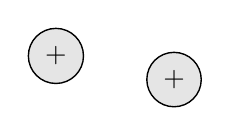
\begin{tikzpicture}
        \node[draw, circle, minimum size = 0.7cm, line width=0.5pt, fill = black!10] at (0,0) {+};
        \node[draw, circle, minimum size = 0.6cm, line width=0.5pt, fill = black!10] at (1.5,-0.3) {+};
    \end{tikzpicture}\\


    Die Wellenfunktionen der Elektronen bei $a$, bzw. $b$ heißen $\phi_\text a$ und $\phi_\text b$, falls die Kerne weit voneinander entfernt sind und sich die Wellenfunktionen nicht gegenseitig beeinflussen.
    Sie befinden sich dann jeweils im Wasserstoffgrundzustand, sind also reele Funktionen.\\
    Die stationäre Schrödingergleichung des Elektrons bei $a$ lautet
    \begin{equation}
        \label{eq:3.1}
        \left( - \frac{\hbar ^2}{2m_0} \Delta - \frac{ \mathrm{e}^2}{4 \pi \varepsilon_0 r_{a}} \right) \varphi_{a} \left( r_{a} \right) = E_{a}^{(0)} \varphi_{a}\left( r_{a} \right),
    \end{equation} 
    $\varphi_\text a$ und die analoge Wellenfunktion $\varphi_\text b$ von Teilchen $b$ sind in \autoref{fig:I.3_wellenfkt_zwei_elektronen_fern} dargestellt.\\
    \begin{figure}[H]
        \centering
        \includegraphics[width=10cm]{figures/vl04/wavefn_two_electrons.png}
        \caption{Wellenfunktionen $\varphi_i$ zweier Elektronen im Wasserstoffgrundzustand an entfernten Positionen $a$ und $b$. Aufgrund des großen Abstandes wechselwirken die beiden Teilchen nicht miteinander.}
        \label{fig:I.3_wellenfkt_zwei_elektronen_fern}
    \end{figure}

    Da beide Wasserstoffatome gleiche sind, ist
    \begin{equation}
        \label{eq:3.2}
        E_{a}^{(0)} = E_{a}^{(0)} = E^{(0)}.
    \end{equation}
    Nähern sich die Kerne an, können die Wasserstoffatome nicht länger als Superposition beider Einzel-Wellenfunktionen betrachtet werden.
    Stattdessen wird die gemeinsame Wellenfunktion $\Psi$ im gemeinsamen Coulombpotential betrachtet. Die neue Schrödingergleichung des Zweiteilchensystems lautet
    \begin{equation}
        \label{eq:3.3}
        \left( - \frac{\hbar ^2}{2 m_0} \Delta - \frac{\mathrm{e}^2}{4 \pi \varepsilon_0 r_{a}} -\frac{\mathrm{e}^2}{4 \pi \varepsilon_0 r_{b}} + \underbrace{\frac{\mathrm{e}^2}{4 \pi \varepsilon_0 R_{ab}}}_{(*)} \right) \psi = E \psi
    \end{equation}
    Der letzte Coulombterm $(*)$ bezieht sich  nicht auf das Elektron und bewirkt lediglich eine Verschiebung der Energieniveaus um einen konstanten Betrag. 
    Dieser Term wird fürs Erste weggelassen und dann später wieder berücksichtigt.\\

    \paragraph{Störungstheorie und LCAO-Methode}
    Zur Lösung dieses Problems wird die {Störungstheorie} verwendet. 
    $\phi_a$ ist weiterhin die ungestörte Wellenfunktion des Elektrons bei $a$.
    Das Coulombpotential von Kern $b$ stört $ \varphi_\text{a} $ und damit $E_\text{a}^{(0)}$ etwas. 
    Das selbe gilt analog für $ \varphi_\text{b}$ und $E^{(0)}_\text{b}$. 
    Die Störung hebt die Entartung der beiden Energiezustände auf.\\

    Nach \quickdef{LCAO-Methode (engl. linear combination of atomic orbitals)} ist der Gesamtzustand $\Psi$ eine Superposition der Einzelzustände
    \begin{equation}
        \label{eq:3.4}
        \psi = c_1 \varphi_{a} + c_2 \varphi_{b}.
    \end{equation}
    Dieser Superpositionsansatz liefert in der Schrödingergleichung \eqref{eq:3.3}
    \begin{equation}
        \label{eq:3.5}
        \begin{aligned}	
        &\left( \underbrace{- \frac{\hbar ^2}{2 m_0} \Delta - \frac{\mathrm{e}^2}{4 \pi \varepsilon_0 r_\text{a}}}_{H_{a}} - \frac{\mathrm{e}^2}{4 \pi \varepsilon_0 r_\text{b}} \right) c_1 \varphi_\text{a} \\ 
            +& \left( - \frac{\hbar ^2}{2 m_0} \Delta - \frac{\mathrm{e}^2}{4\pi \varepsilon_0 r_\text{b}} - \frac{\mathrm{e}^2}{4 \pi \varepsilon_0 r_\text{a}} \right) c_2 \varphi_\text b\\
            =& E \left( c_1 \varphi_\text{a}+ c_2 \varphi_\text{b} \right) 
        \end{aligned}
    \end{equation}

    Mit \eqref{eq:3.1}, $H_\text{a} \varphi_\text{a}= E_\text{a}^{(0)} \varphi_\text{a}$, $H_\text{b} \varphi_\text{b}= E_\text{b}^{(0)} \varphi_\text{b}$ und $E^{(0)}_\text{a} = E^{(0)}$ gilt
    \begin{equation}
        \label{eq:3.6}
        \Big( \underbrace{E^{0} -E}_{ \Delta E} - \frac{\mathrm{e}^2}{4 \pi \varepsilon_0 r_\text{b}}  \Big) c_1 \varphi_\text a + \Big( \underbrace{E^{0} -E}_{ \Delta E} - \frac{\mathrm{e}^2}{4 \pi \varepsilon_0 r_\text{a}} \Big) c_2 \varphi_\text{b} =0
    \end{equation}
    $\varphi_\text{a}$ und $\varphi_\text{b}$ sind Funktionen des Orts $r_\text{a,b}$, $c_1$ und $c_2$ sind ortsunabhängige komplexe Konstanten.
    Durch Multiplikation mit $\varphi^*_\text a$ und $\varphi^*_\text b$ und Integration über die Elektronenkoordinate $\mathrm d^3r = \text dV$ erhält man aus Gleichung \eqref{eq:3.6} vier unterschiedliche Integrale:
    
    \stepcounter{equation}
    \begin{align}
        \nonumber
        &\int \varphi_\text{a} \varphi_\text{b} \mathrm{d}V = 1\\
        \nonumber
        &\int \varphi_\text{a} \varphi_\text{b} \mathrm{d}V = S &&\text{(Überlappintegral)}\\
        \label{eq:3.8}
        &\int \varphi_\text{a} \left( r_\text{a} \right) \left( - \frac{\mathrm{e}^2}{4\pi \varepsilon_0 r_\text{b}}  \right) \varphi_\text{a}\left( r_\text{a} \right) \mathrm{d}V = C &&\text{(Coulombintegral)} \\
        \label{eq:3.9}
        &\int \varphi_\text{a} \left( r_\text{a} \right) \left( - \frac{\mathrm{e}^2}{4 \pi \varepsilon_0 r_\text{a}}  \right) \varphi_\text{b}\left( r_\text{b} \right) \mathrm{d}V = D &&\text{(Austauschintegral)}
    \end{align}
    Beachte: $ \varphi_\text{a}$ und $ \varphi_\text{b}$ sind nicht orthogonal, also $ S\neq 0$. 
    Die physikalische Bedeutung des Coulombintegrals \eqref{eq:3.8} ist in \autoref{fig:I.3_wellenfkt_zwei_elektronen_fern} dargestellt.\\
    
    \begin{figure}[H]
        \centering
        \includegraphics[width=10cm]{figures/vl04/wavefn_coulomb_integral.png}
        \caption{Coulomb'sche Wechselwirkung zwischen $e\varphi_\text a^2$ und dem Coulombfeld von Teilchen $b$. $-e\phi^2_\text a$ hat dabei die Bedeutung der Ladungsdichte des Elektrons.}
        \label{fig:I.3_wavefn_coulomb_integral}
    \end{figure}

    Die physikalische Bedeutung des Austauschintegrals \eqref{eq:3.9} ist in \autoref{fig:I.3_wavefn_exchange_integral} dargestellt.

    \begin{figure}[H]
        \centering
        \includegraphics[width=10cm]{figures/vl04/wavefn_exchange_integral.png}   
        \caption{Wellenfunktionen $\varphi_i$ zweier Teilchen an $a$ und $b$ im Coulomb-Potential (blau). $e\varphi_\text a\varphi_\text b$ bedeutet, dass das Elektron sich gewissermaßen teilweise im Zustand $\phi_\text a$, teilweise im Zustand $\phi_\text b$ aufhält, oder mit anderen Worten ein \textbf{Austausch} zwischen diesen beiden Zuständen vorkommt.}     
        \label{fig:I.3_wavefn_exchange_integral}
    \end{figure}

    Multiplizieren wir Gleichung \eqref{eq:3.6} mit $ \varphi^{*}_\text{b}$ statt mit $ \varphi_\text{a}^{*}$, führt das zu ähnlichen Ausdrücken. 
    \eqref{eq:3.6} geht über in
    \begin{align}
        \label{eq:3.10}
        \left( \Delta E + C \right) C_1 + \left( \Delta E S + D \right) C_2 &= 0, \\
        \label{eq:3.11}
        \left( \Delta E S + D \right) C_1 + \left( \Delta E + C \right) C_2 &= 0.
    \end{align}
    Es handelt sich hierbei um 2 Gleichungen mit 2 Unbekannten, d.h. die Determinante muss verschwinden:
    \begin{equation}
        \label{eq:3.12}
        \left( \Delta E + C \right) ^2 - \left( \Delta ES + D \right) ^2 = 0
    \end{equation}
    \begin{equation}
        \label{eq:3.13}
        \Rightarrow \left( \Delta E + C  \right) = \pm \left( \Delta ES + D \right) 
    \end{equation}
    Setze \eqref{eq:3.13} in \eqref{eq:3.10} bzw. \eqref{eq:3.11} ein:
    \begin{equation}
        \label{eq:3.14}
        C_2 = - C_1 = -C
    \end{equation}
    Somit erhalten wir die Gesamtwellenfunktionen
    \begin{align}
        \label{eq:3.15}
        \Rightarrow \psi_{-} &= c\left( \varphi_\mathrm{a} - \varphi_\mathrm{b} \right) \qquad\text{antisymmetrisch und} \\
        \label{eq:3.16}
        \psi_{+} &= c\left( \varphi_\mathrm{a} + \varphi_\mathrm{b} \right) \qquad\text{symmetrisch,}
    \end{align}
    welche in \autoref{fig:I.3_wavefn_Psi_plus_minus} skizziert sind.

    \begin{figure}[H]
        \centering
        \includegraphics[width=8cm]{figures/vl04/wavefn_Psi_plus_minus.png}
        \caption{Gesamtwellenfunktionen $\Psi_-$ nach \eqref{eq:3.15} und $\Psi_+$ nach \eqref{eq:3.16} als antisymmetrische, bzw. symmetrische Überlappung der Einzelzustände $\varphi_\mathrm a$ und $\varphi_\mathrm b$.}
        \label{fig:I.3_wavefn_Psi_plus_minus}
    \end{figure}

    Die Energien in diesen Zuständen sind
    \begin{align}
        \label{eq:3.17}
        E^{(-)} &= E_{0} + \frac{C-D}{1-S} \quad 0 < S < 1 \\
        \label{eq:3.18}
        E^{(+)} &= E_0 + \frac{C+D}{1+S}\quad C, D \le 0.
    \end{align}
    Um zu entscheiden ob eine Bindung zustandekommt, muss man die Energie bei endlichem Abstand mit der bei unendlichem Abstand $\left( C= D = 0 \right) $ vergleichen und noch die Coulomb-Abstoßungsenergie der Kerne mit $ E^{+}$ und $E^{-}$ berücksichtigen, womit 
    $$
    E_{\text{Bindung}} = \frac{C \pm D}{1 \pm S} + \frac{\mathrm{e}^2}{4 \pi \varepsilon_0 R_\mathrm{a,b}}
    \begin{cases}
        < 0 &\text{bindend}\\
        > 0 &\text{antibindend}
    \end{cases}
    $$ 
    folgt. $C$ lässt sich auch als Funktion von $R_\mathrm{a,b}$ analysieren:
    \begin{itemize}
        \item ist $R_\mathrm{a,b}$ deutlich größer als die Ausdehnung von $ \varphi_\mathrm{a}$ oder $ \varphi_\mathrm{b}$, so gilt $C \approx E_{\text{pot}}$ einer Punktladung im Feld des anderen Kerns und
            $$
            C \approx - \frac{\mathrm{e}^2}{4 \pi \varepsilon_0 R_\mathrm{a,b}}
            $$
        \item Für $R_\mathrm{a,b}\to 0$ geht die Coulomb'sche Abstoßungsenergie gegen unendlich, aber $C$ wird endlich negativ:
            $$
            \to C + \frac{\mathrm{e}^2}{4\pi \varepsilon_0 R_\mathrm{a,b}}>0 \quad \to \quad \text{keine Bindung!}
            $$ 
    \end{itemize}

    Auch $D$ lässt sich als Funktion von $R_\mathrm{a,b}$ analysieren:
    \begin{itemize}
        \item Für $R_\mathrm{a,b}\to 0 $ geht $ \varphi_\mathrm{a}$ in $ \varphi_\mathrm{b}$ über, d.h. es gilt $ D= C$. Somit kann die Coulomb'sche Abstoßungsenergieder der Kerne nicht kompensiert werden.
        \item Für wachsendes $R_\mathrm{a,b}$ nehmen sohwohl
            $$
            \frac{\mathrm{e}^2}{4 \pi \varepsilon_0 R_\mathrm{a,b}}, 
            $$ 
            als auch $D$ (mit entgegengesetzten Vorzeichen), dem Betrag nach ab.
    \end{itemize}
    Numerische Berechnungen zeigen, dass für bestimmte $R_\mathrm{a,b}$ die Bindungsenergie $E_{\text{bind}}$ positiv wird.

    \begin{important}\unboldmath
        \textbf{Faustregel Bindungseffekt}\\[1ex]
        Der Bindungseffekt beruht entscheidend auf dem Auftreten der Austauschdichte $\varphi_\mathrm{a}^{*} \varphi_\mathrm{b}$ im Term $D$. 
        Es handelt sich um einen \textbf{quantenmechanischen Effekt}!
    \end{important}

    Nach diesem Modell beträgt die Bindungsenergie im Wasserstoffion \ce{H2+} 
    $$E^\mathrm{Modell}_\mathrm{bind}=\SI{1.7}{\electronvolt}.$$
    Experimentell wird jedoch ein Wert von 
    $$E^\mathrm{exp}_\mathrm{bind}=\SI{2.6}{\electronvolt}$$
    gemessen. Das Modell weicht also stark vom Messwert ab. Als verbesserter Ansatz kann
    $$\Psi = C\left[\exp\left(\frac{-\alpha r_\mathrm a}{a_0}\right) + \exp\left(\frac{-\alpha r_\mathrm b}{a_0}\right) \right]
    $$
    gewählt werden, mit dem Bohr'schen Radius $a_0$ und dem Variationsparameter $\alpha$, welcher für $\alpha=1,24$ die besten Vorhersagen trifft.
    
    \begin{minipage}{0.4\linewidth}
         Durch den Variationsparameter wird ein effektiv kleinerer Bohrradius gewählt und die Elektronenwelle senkrecht zur Verbindungslinie zwischen den Kernen zusammengedrückt.
    \end{minipage}
    \hspace{0.8cm}
    \begin{minipage}{0.52\linewidth}
        \centering
        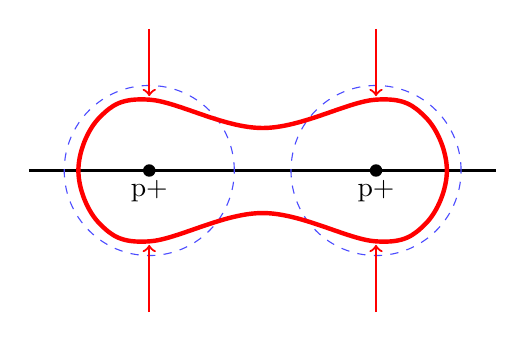
\begin{tikzpicture}[scale=0.9]

            % --- Grundlinie und Punkte ---
            \draw[thick] (-3.3,0) -- (3.3,0);
            \fill (-1.6,0) circle (2.5pt) node[below] {\ce{p+}};
            \fill ( 1.6,0) circle (2.5pt) node[below] {\ce{p+}};

            % --- blaue kreise
            \draw[blue!70, dashed] (-1.6,0) circle (1.2);
            \draw[blue!70, dashed] ( 1.6,0) circle (1.2);

            % --- rote pfeile
            \draw[red, ->, thick] (-1.6, 2) -- (-1.6, 1.05);
            \draw[red, ->, thick] (-1.6,-2) -- (-1.6,-1.05);
            \draw[red, ->, thick] ( 1.6, 2) -- ( 1.6, 1.05);
            \draw[red, ->, thick] ( 1.6,-2) -- ( 1.6,-1.05);

            % --- rote linie
            \draw[red,ultra thick] plot [smooth cycle, tension = 0.62]
            coordinates {
                (-2.6,0) (-2.3,-0.75) (-1.6,-1.0) (0,-0.6) 
                (1.6,-1.0) (2.3,-0.75) (2.6,0) (2.3,0.75) (1.6,1.0) (0,0.6) 
                (-1.6,1.0) (-2.3,0.75)
            };
        \end{tikzpicture}
        \captionof{figure}{Zusammengedrückte Elektronenwelle im \ce{H2}-Molekül durch Wahl eines Variationsparameters $\alpha>1$.}
    \end{minipage}


    